\documentclass{article}
    \usepackage{multicol}
    \usepackage[fontset = windowsnew, heading = true, hyperref]{ctex}
    \ctexset{paragraph/beforeskip=0.5ex, section/beforeskip=1ex, section/afterskip=0.5ex, subsection/beforeskip=1ex, subsection/afterskip=0.5ex, subsubsection/beforeskip=1ex, subsubsection/afterskip=0.5ex}
    \pagestyle{plain}
    \usepackage{geometry}
        \geometry{left=2cm,right=2cm,top=2cm,bottom=2cm}
    \usepackage{amsmath}
    \usepackage{amsfonts}
    \usepackage{siunitx}
    \usepackage{booktabs}
    \usepackage{longtable}
    \usepackage{graphicx}
    \usepackage{subfig}
    \usepackage{float}
    \usepackage{fancyvrb}
    \renewcommand{\labelenumi}{\alph{enumi}.} % Make numbering in the enumerate environment by letter rather than number

    \setlength{\parskip}{0pt}
    \setlength{\parsep}{1ex}
    \linespread{1.1}

    \title{\textbf{基于视听信息的视频分类标注系统设计} \\ [1.5ex] \begin{large} \emph{结题报告} \end{large} }
    \author{王晗 \\ (2013011076) \\ 清华大学电子工程系无32班 \\ han-wang@outlook.com
            \and
            宗卉轩 \\ (2013011052) \\ 清华大学电子工程系无32班 \\ zonghx13@mails.tsinghua.edu.cn}
    \date{}

\begin{document}
    \maketitle

\begin{multicols}{2}
    \section{成员及分工}
        \paragraph{王晗}
        服务器搭建、视觉特征提取、模型设计、模型训练、测试验证、报告主笔

        \paragraph{宗卉轩}
        听觉特征提取、模型训练、报告听觉特征部分撰写

    \section{文件清单}
        文件清单如表\ref{tabel:filelist}所示,未列在文件清单中的工程文件保持原始状态,提交文件中不包括数据集和mexopencv、mmread、FFGrab。
        \begin{table*}[htb]
          \centering
          \begin{tabular}{lll}
            \toprule
            \textbf{Directory} & \textbf{File} & \textbf{Description} \\
            \midrule
            /workspace  & /run\_project\_test.m & 基于测试集的主程序 \\
                        & /fun\_process.m & 视频分类处理函数 \\
                        & /processVideo.m & 视觉特征提取 \\
                        & /processAudio.m & 听觉特征提取 \\
                        & /processObject.m & 内容特征提取 \\
                        & /fun\_datagen.m & 视听特征分段生成工具 \\
                        & /run\_objectdata.m & 内容特征分段生成工具 \\
                        & /run\_datacompose.m & 分段数据合成工具 \\
                        & /run\_predictorcompress.m & 特征压缩工具 \\
                        & /run\_modelgen.m & 预测模型生成工具 \\
                        & /data/baggedtree.mat & Bagged Tree模型 \\
                        & /data/auxilary.mat & 辅助数据 \\
                        & /data/frontalface.xml & 人脸级联检测器 \\
            \midrule
            /dataset    & /TRAINset.mat & 从Blip10000中划分的训练集 \\
                        & /TESTset.mat & 从Blip10000中划分的测试集 \\
            \midrule
            /report     & /report.pdf & 设计报告(本文档) \\
            \bottomrule
          \end{tabular}
          \caption{文件清单}
          \label{tabel:filelist}
        \end{table*}

    \section{基本需求部分}
        \subsection{基本原理}
            我们选定如下的基于视听信息的特征来描述视频\cite{webvideo}:
            \paragraph{听觉特征}
            时频谱特征(Spectral Pattern)、差分时频谱特征(Delta Spectral Pattern)、方差量化的差分时频谱特征(Variance Delta Spectral Pattern)、基于时频谱的波动谱特征(Fluctuation Pattern)、相关谱特征(Correlation Pattern)、时频谱极值特征(Spectral Contrast Pattern)、短时过零率(Short-time zero crossing rate)、均方能量(Square mean energy)
            \paragraph{时间特征}
            平均节奏(Rhythm)、快节奏比例(Hot Action Rate)、慢节奏比例(Cold Action Rate)、 渐变比例(Gradual Transition Rate)
            \paragraph{颜色特征}
            全局颜色直方图(Global Weighted Color Histogram)、基本颜色直方图(Elementary Color Histogram)、 颜色性质(Color Properties)等。

            基于从Blip10000中随机划分的训练集,利用Matlab R2015b 中的Neural Network工具箱、Ensemble Learning 工具箱和Classification Learner工具箱\footnote{Classification Learner工具箱仅在Matlab R2015a及以后版本可用。}分别建立神经网络模型、Bagged Tree模型和SVM模型,使用上述特征训练分类器。对于测试集中待分类的视频,同样提取上述特征,使用分类器进行分类。

            \subsubsection{听觉特征}
                \paragraph{时频谱特征}
                短时傅里叶变换,反映了大约0.2s内的音色特征。
                \paragraph{差分时频谱特征}
                考虑到声音的端点,反映了大约0.5s内的时频谱差分特征。
                \paragraph{方差量化的差分时频谱特征}
                提取端点的强度随时间变化的特征,反映了声音的连续性。
                \paragraph{基于时频谱的波动谱特征}
                声音的周期特性,反映了大约6s内的节奏特征。
                \paragraph{相关谱特征}
                频率的相关性分析,反映了不同音色和节奏之间的时域关系。
                \paragraph{时频谱极值特征}
                较短的一段时间内声音的频率范围,反映了音域特征。

            \subsubsection{时间特征}
                根据直接剪切、淡入淡出、溶解划分场景,据此计算以下特征:
                \paragraph{平均节奏}
                平均每个场景的持续时间,反映了视频的整体节奏。
                \paragraph{快节奏比例}
                持续时间小于等于3s的场景在所有场景中所占比例,反映了视频的紧张程度。
                \paragraph{慢节奏比例}
                持续时间大于等于8.3s的场景在所有场景中所占比例,反映了视频的舒缓程度。
                \paragraph{渐变比例}
                淡入淡出、溶解过程占视频全长的比例,反映了视频的剪辑效果。

            \subsubsection{颜色特征}
                真彩色颜色空间较大,不便于计算,因此我们将颜色压缩映射到Web安全色(216色)空间中,这同时可以减小噪声的影响。

                \paragraph{全局颜色直方图}
                对每个场景的颜色直方图进行加权平均,权重为场景长度占视频全长的比例。

                \paragraph{基本颜色直方图}
                根据主观色彩分类,将Web安全色映射为10种基本色系,计算其分布直方图。

                \paragraph{颜色性质}
                根据主观色彩分类,将Web安全色分为深色/浅色、冷色/暖色、灰白色、对比色、相似色,分别计算其比例。

                这些颜色特征可以反映视频给人的主观色彩感受。

        \subsection{具体实现}
            \subsubsection{计算听觉特征}
                首先判断音频长度。如果时间大于6分钟,则取音频中间长度合适的一部分;如果时间小于1分钟,为了能够得到足够的相应的特征,把spectrogram函数的帧长减小为正常的1/4。然后判断音频数据是否为全0,若为0 则把所有的特征向量赋0,退出程序。接着把采样率高的音频重新采样,减少数据量的同时使得各个特征的维度保持一致。

                使用MATLAB自带的spectrogram函数生成所需要的时频谱,对生成的矩阵依次进行取绝对值、高频部分压缩、减去邻域平均值的步骤得到可以提取音频特征的时频谱。

                沿着时间轴把时频谱分块,对块进行处理。然后应用量化函数从每个块里提取相应的谱特征,块的大小和是否重叠都由需要提取的特征来决定。

                上述步骤之后得到每个谱特征的一个特征矩阵,而要得到特征向量,我们目前的做法是取均值。这样做减小了数据,也不失为一种相对稳妥的量化方法。在提高部分,针对不同的谱特征,我们会尝试使用各种不同的量化方法来得到特征向量以求更精确的反应音频特征。

                除了上述时频谱特征外,还计算了短时过零率和均方能量这两个比较重要的时域特征。

            \subsubsection{视频读取策略}
                为了减小计算量,我们控制最高读取帧率10FPS,周期和人眼的视觉暂留时间相同。读入的RGB图像经过缩放,再转换为HSV色彩模式。

                由于将视频逐帧转换为图像、保存至硬盘、从硬盘读入的过程受到解码速度、硬盘I/O速度的制约,非常缓慢,并且会消耗巨大的硬盘空间,我们采用了两种不同的策略进行视频读取:

                \paragraph{训练视频}
                我们不进行视频到图片的逐帧转换,而是根据filename 域直接读取视频,每读入100帧并进行压缩,再读入100 帧,以此类推。对于持续时间过长的视频,我们仅在内存中保留视频中间的5分钟,我们可以认为视频的主要内容集中在视频持续时间的中段,这样的截取操作可以在减小计算量的同时不影响视频主题的判断。

                \paragraph{测试视频}
                由于现有框架下视频到图片的逐帧转换不计入测试时间,而这一过程包括了消耗时间巨大的视频解码工作,因此我们只能使用原框架中的逐帧转换过程,牺牲硬盘空间和I/O速度,从而换取解码时间的排除。

            \subsubsection{场景划分}
                我们寻找如下三种场景切换点:

                \paragraph{淡入淡出}
                在V平面计算亮度方差,若检测到小于阈值0.006的帧,则向前后查找淡入淡出的入点和出点,并将当前点记为场景分割点。

                \paragraph{直接剪切}
                使用OpenCV中的Canny函数查找边缘,计算相邻两帧边缘像素的出入率ECR,并使用Matlab中的FindPeaks 函数查找峰值,确定场景分割点。

                \paragraph{溶解过渡}
                对亮度方差求二阶导数,查找连续的大于0的区间,确定溶解过程和场景分割点。

            \subsubsection{计算视觉特征}
                使用上节所述的定义计算各视觉特征,其中全局颜色直方图使用OpenCV中的calcHist函数实现。

        \subsection{性能分析}
            \paragraph{听觉特征}
            截取音频数据长度为$N$,频带数目为$L$。调用spectrogram函数复杂度为$O(LN^2)$。SP、DSP、VDSP的复杂度为$O(LN)$。FP、SCP的复杂度为$O(LN^2)$。CP的复杂度为$O(L^2N)$。短时过零率和均方能量的复杂度分别为$O(N^2)$和$O(N)$。

            \paragraph{视觉特征}
            设画面边长为$N$,视频长度为$L$。场景分割需要对视频进行一次遍历,每一帧需要像素点级的处理,因此复杂度为$O(LN^2)$。时间特征计算的复杂度为$O(L)$。颜色特征中,全局颜色直方图计算的复杂度为$O(LN^2)$,其他颜色特征均为$O(1)$。视觉特征处理的复杂度和听觉特征相比较高,算法优化的重点应当在于视觉部分。

            \paragraph{实际性能}
            实际测量结果表明,我们的程序处理一个视频的时间和视频实际时长可以相比(约0.2倍视频原长),具有良好的分类效率。程序执行的大部分时间花费在磁盘I/O操作中。为了减少I/O速度对计算速度的影响,我们尽可能减少磁盘读取次数,例如降低读取帧率,将帧图像缓存在内存中,同时进行淡入淡出、直接剪切、溶解过渡的检测,使用抽样方法计算颜色直方图等。除此之外,耗费时间最多的是RGB转HSV颜色模式、亮度方差计算等过程,因此我们在读取视频的同时,对读入的帧图像进行了缩放,减小内存消耗和后续处理过程的计算量。

            在分类精确度方面,由于样本数量较少,神经网络模型无法取得较好的效果,而SVM和Bagged Tree在样本较少时也具有较好的分类效果。

        \subsection{问题与不足}
            \paragraph{分类精确度}
            目前分类精确度在不同类别中差异较大,在提高部分我们需要考虑有针对性地予以增强。

            \paragraph{模型动态更新}
            fun\_process.m函数每次调用时会传入上一个视频的正确分类,我们目前还没有利用这一信息实现分类模型的动态更新,这是我们在提高部分要重点探究的内容。

    \section{提高需求部分}
        \subsection{原理和实现}
            \subsubsection{特征压缩}
                基本要求部分特征(Predictors)过多,而样本数量相对不足,造成机器学习结果并不理想。我们考虑对维度较高的全局颜色直方图和部分音频特征进行压缩。

                \paragraph{星座距离}
                我们对每一个类别的$SP,DSP,VDSP,\\ LFP,CP,H_{gw}$特征求取平均,得到一组向量,称它为每一个类别的星座。任意一个视频的全局颜色直方图均可以定义它到不同星座的距离。这里我们采用欧氏距离,即:
                $$d=\sqrt{\sum_{i}(H_i-\bar{H}_i)^2}$$

                \paragraph{颜色熵}
                由于熵的定义为
                $$H=-\sum_i p_i\log_2 p_i$$
                我们可以根据各种颜色在全局颜色直方图中出现的概率计算颜色熵。

                \paragraph{音频带宽}
                我们将音频信号看作低通信号,定义70\%总能量占据的频率区间为音频带宽。

            \subsubsection{基于内容理解的分类增强}
                中期检查结果表明,基本要求部分在不同类别的分类中精确度差异较大。因此我们考虑使用OpenCV中的Haar特征级联分类器对视频内容进行识别。目前人脸检测的研究较多,我们使用了Itseez的训练样本
                \footnote{来源:https://github.com/Itseez/opencv/tree/master/data/haarcascades}。我们也尝试了对半身人像、全身人像、乐器(吉他/钢琴)、话筒等物体进行检测,但受限于正反样本数量过少,检测结果并不理想。我们进而对斑点、角点等图像基元的检测,用以替代物体检测。

                \paragraph{人脸特征}
                不同类别的视频中,人脸的数量、占据画面的比例等存在较大差异。因此我们在视频中的不同位置等概率提取不超过31帧图像,使用Haar特征级联分类器进行人脸检测。分别计算最大的人脸和所有人脸占据画面的比例、人脸数量、不同画面中人脸的比例等特征。

                \paragraph{斑点特征}
                不同分类的视频中,灰度变化明显的区域存在一定差别,我们使用OpenCV中的Feature Detector对斑点进行检测,以斑点的平均数量和面积比例作为特征。

                \paragraph{角点特征}
                我们尝试过物体检测和广义哈夫变换进行图形检测,其召回率过低,效果均不理想。最后我们决定使用角点特征代替。使用OpenCV中的cornerHarris算法对灰度图像进行处理,经过归一化后,再使用ConvertScaleAbs转换为无符号整形,得到角点的位置,以角点平均数量作为特征。

            \subsubsection{分类结果反馈更新}
                我们使用全局变量记录了上一个视频的\\$SP, DSP, VDSP, LFP, CP, H_{gw}$特征以及预测的分类结果,和输入的正确分类结果进行比较,采用老化算法,以该类别已有的样本数为年龄,按照
                $$S_{true,new}=S_{true}+\mathbf{e}/age$$
                对星座坐标进行更新,其中$\mathbf{e}=Feature-S_{true}$为误差向量。

        \subsection{性能分析}
            \paragraph{特征压缩}
            对视听特征的压缩均为$O(1)$复杂度,而特征压缩会使得预测模型的复杂度减小,从而带来整体性能的提升。

            \paragraph{新增特征}
            新增加的视觉特征仅在视频中不同位置采样提取,采样数量固定,因此和视频长度无关,仅和画面尺寸相关。由于我们对图像进行了缩放处理,因此复杂度也可近似为$O(1)$。

            \paragraph{星座坐标更新}
            由于星座数量固定,因此星座坐标更新过程的复杂度为$O(1)$。

            \paragraph{实际性能}
            经过采样处理、特征压缩后,我们的时间效率较高,处理一段视频的相对时间约为0.5。Bagged Tree预测模型交叉验证给出的Confusion Matrix 如图\ref{fig:confusionmatrix}所示,整体准确率可以达到74.2\%,Politics 类别视听特征突出,提高部分的人脸检测也对该类别进行了优化,因此准确率达到90.5\%;Musics类别的听觉特征明显,分类准确率也较高;Sports类别的准确率由中期检查时的约14\%提升至21.9\%。
            
            \begin{figure}[H]
              \centering
              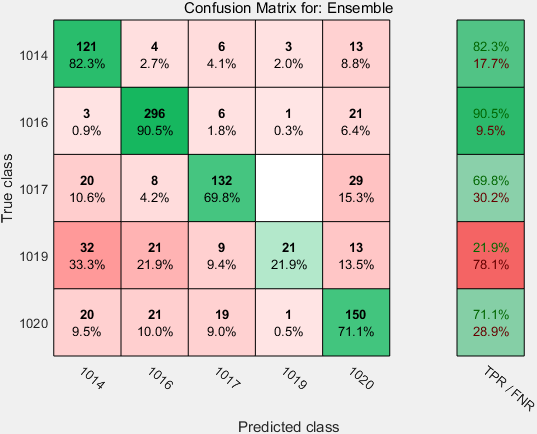
\includegraphics[width=7.4cm]{confusionmatrix.png}
              \caption{Confusion Matrix}\label{fig:confusionmatrix}
            \end{figure}

        \subsection{问题与不足}
            \paragraph{Matlab版本}
            我们的程序主要基于Matlab R2015b平台完成,个别功能在R2015a以后发生了变化,因此在旧版平台运行时可能会出现警告或错误。

            \paragraph{OpenCV崩溃}
            OpenCV 3.0中的Feature Detector提供了多种算法,不同算法崩溃概率不同,目前使用的SimpleBlob算法在970 个训练样本中发生了一次崩溃。尚不清楚发生崩溃的原因,可能和OpenCV或mexOpenCV的内存管理有关。
            
            \paragraph{Sports类别准确率较低}
            该类别中包括比赛录像、人物访谈、新闻报道、音乐相册等多种类型的视频,缺乏统一特征,在视听信息层面和其他类别有较多重叠,因此分类准确率较低。该类别可用于训练的样本非常少,进一步恶化了该类别的分类效果。相关文献报道的Sports类别准确率也仅有30\%-40\%,对该问题的改善可能需要更深入的语义理解等方法,而非仅仅依赖视听信号特征。

    \section{总结与收获}
        以中期检查为分界线,前半学期我们根据文献\cite{webvideo}提取基本的视听特征,尝试使用ANN、Bagged Trees、SVM 等机器学习方法进行训练,搭建起了本次大作业的完整框架,但是存在分类正确率较低、分类器体积庞大等问题。中期检查以后的工作基本为原创性质,我们提出了星座距离方法实现了对视听特征的有效压缩,并且通过星座坐标的更新实现了模型的动态反馈调整。我们还加入了人脸、斑点、角点检测等处理,增强了分类准确率。Bagged Tree模型的交叉验证给出整体准确率达到74.2\%,而中期检查时最薄弱的Sports分类也有所提升。

        这次大作业让我们对时频谱、短时过零率、颜色直方图、颜色熵、SIFT等视听特征有了直观的认识,提取并应用的过程又进一步加深了我们的理解。这次大作业中需要使用OpenCV和机器学习方法,对它们的学习开阔了我们的视野,也让我们能够通过这次大作业接触到图像、音频处理领域的前沿。


    \bibliographystyle{plain}
    \bibliography{ref.bib}

\end{multicols}


\end{document}
